% !TeX root = ../main.tex
% Add the above to each chapter to make compiling the PDF easier in some editors.

\chapter{Homomorphism and Isomorphism Theorems}
In this chapter, we will discuss tools to show that two groups are isomorphic.

\begin{thm}[Homomorphism Theorem]\index{homomorphism theorem}
Let $\varphi : G \to H$ be a group homomorphism. Then, \begin{align}
    \rep{\varphi} : \Quot{G}{\ker{\varphi}} \to \im{\varphi},\quad a \ker{\varphi} \mapsto \varphi(a)
\end{align} is an isomorphism. Especially, $\Quot{G}{\ker{\varphi}} \isom \im{\varphi}$.
\end{thm} \begin{proof}
\leavevmode\begin{itemize}
    \item We will first show that $\rep{\varphi}$ is well-defined. For any $a, b \in G$, \begin{align*}
        &a \ker{\varphi} = b \ker{\varphi} \\
        \iff\quad &\inv{a} b \in \ker{\varphi} \margintag{by \cref{lem:cosets_eq}} \\
        \iff\quad &\varphi(\inv{a} b) = e_H \margintag{using the definition of the kernel \eqref{eq:kernel}} \\
        \iff\quad &\inv{\varphi(a)} \varphi(b) = e_H \margintag{using that $\varphi$ is a homomorphism \eqref{eq:homomorphism}} \\
        \iff\quad &\varphi(a) = \varphi(b) \\
        \iff\quad &\rep{\varphi}(a \ker{\varphi}) = \rep{\varphi}(b \ker{\varphi}). \margintag{using the definition of $\rep{\varphi}$}
    \end{align*} The direction ``$\Rightarrow$'' shows that $\rep{\varphi}$ is well-defined. Note that ``$\Leftarrow$'' shows that $\rep{\varphi}$ is injective.
    
    \item Next, we show that $\rep{\varphi}$ is a homomorphism. For any $a, b \in G$, \begin{align*}
        \rep{\varphi}(a \ker{\varphi} \cdot b \ker{\varphi}) &= \rep{\varphi}(a b \ker{\varphi}) \margintag{using the operation of the quotient group \eqref{eq:quotient_group_op}} \\[5pt]
        &= \varphi(a b) \margintag{using the definition of $\rep{\varphi}$} \\
        &= \varphi(a) \cdot \varphi(b) \margintag{using that $\varphi$ is a homomorphism \eqref{eq:homomorphism}} \\
        &= \rep{\varphi}(a \ker{\varphi}) \cdot \rep{\varphi}(b \ker{\varphi}). \margintag{using the definition of $\rep{\varphi}$}
    \end{align*}
    
    \item Finally, we observe that $\rep{\varphi}$ is surjective. That is, for any $a \in \im{\varphi}$, we have that $a \ker{\varphi} \in \Quot{G}{\ker{\varphi}}$. \qedhere
\end{itemize}
\end{proof}

\begin{ex}{Homomorphism theorem}{}
We have already seen in \cref{ex:homomorphisms} that for any field $K$, ${\det : \GL{n}{K} \to \woZ{K}}$ is a homomorphism with ${\ker{\det} = \SL{n}{K}}$. Thus, by the homomorphism theorem, \begin{align}
    \Quot{\GL{n}{K}}{\SL{n}{K}} \isom \woZ{K}.
\end{align}
\end{ex}

\begin{marginfigure}
    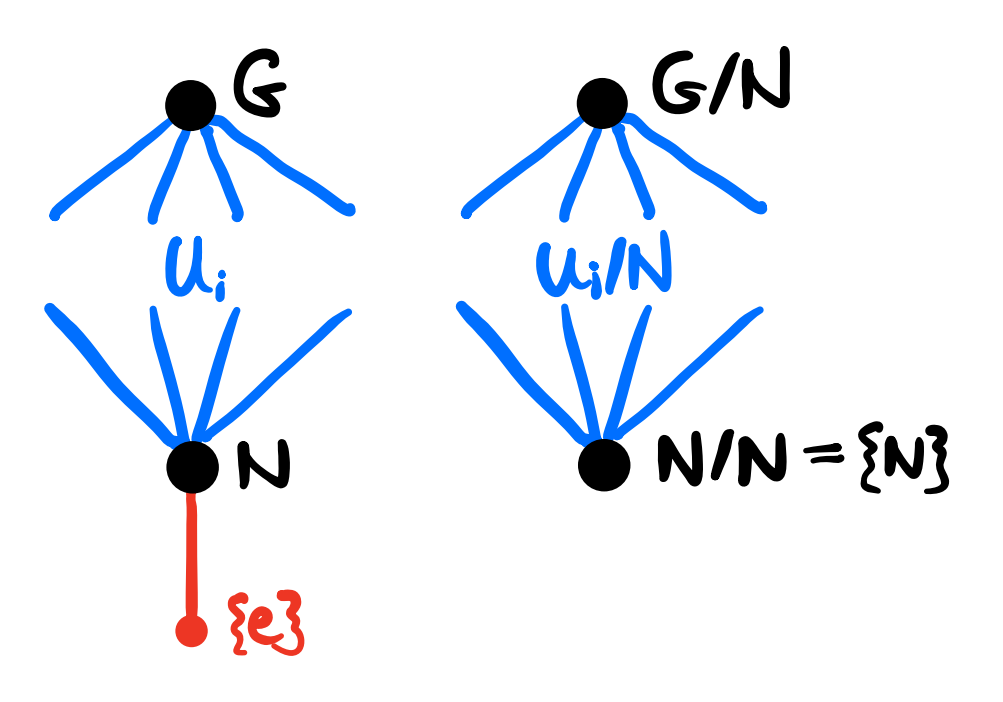
\includegraphics[width=\textwidth]{correspondence_thm.png}
    \caption{Sketch of the correspondence of subgroups $U_i$ ``between'' $G$ and $N$ and the subgroups $\Quot{U_i}{N}$ ``between'' $\Quot{G}{N}$ and $\Quot{N}{N}$.}\label{fig:correspondence_thm}
\end{marginfigure}

\begin{thm}[Correspondence Theorem]\index{correspondence theorem}
The mapping, \begin{align}
    f : \{U \subgroup G \mid N \subseteq U\} \to \{V \subgroup \Quot{G}{N}\},\quad U \mapsto \Quot{U}{N},
\end{align} is an inclusion-preserving\footnote{We say that a mapping ${f : A \to B}$ is \emph{inclusion-preserving}\index{inclusion-preserving mapping} if for any $a_1, a_2 \in A$ such that ${a_1 \subseteq a_2}$, we have ${f(a_1) \subseteq f(a_2)}$.} bijection and fore every $U \subgroup G$, \begin{align}
    U \normal G \iff \Quot{U}{N} \normal \Quot{G}{N}.
\end{align}
\end{thm} \noindent A sketch of the correspondence theorem is given in \cref{fig:correspondence_thm}.

\begin{marginfigure}
    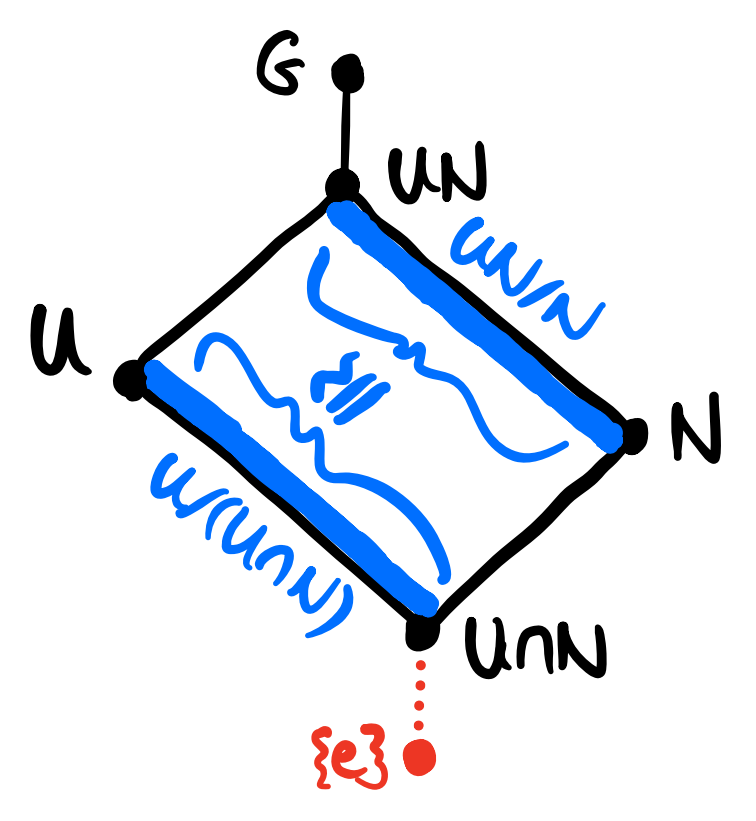
\includegraphics[width=\textwidth]{first_isom_thm.png}
    \caption{Sketch of the first isomorphism theorem.}\label{fig:first_isom_thm}
\end{marginfigure}

\begin{thm}[First Isomorphism Theorem]\index{first isomorphism theorem}\index{isomorphism theorem}
Let $U \subgroup G$ and $N \normal G$. Then, \begin{thmlist}
    \item $U N \subgroup G$ where $U N \defeq \{x \cdot n \mid x \in U, n \in N\}$
    \item $U \cap N \normal U$
    \item $\Quot{UN}{N} \isom \Quot{U}{(U \cap N)}$
\end{thmlist}
\end{thm} \noindent A sketch of the correspondence theorem is given in \cref{fig:first_isom_thm}.

\begin{marginfigure}
    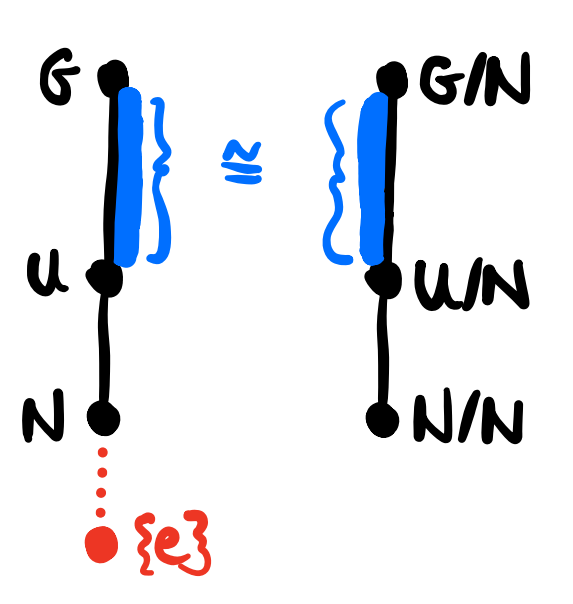
\includegraphics[width=\textwidth]{second_isom_thm.png}
    \caption{Sketch of the second isomorphism theorem..}\label{fig:second_isom_thm}
\end{marginfigure}

\begin{thm}[Second Isomorphism Theorem]\index{second isomorphism theorem}\index{isomorphism theorem}
Let $U, N \normal G$ with $N \subseteq U$. Then, $\Quot{(\Quot{G}{N})}{(\Quot{U}{N})} \isom \Quot{G}{U}$.
\end{thm}